\classheader{10-09-2017}

\definition{A topological space $X$ is \textbf{locally connected} at $x$ if every open set $U$ containing $x$ has the property that there exists a $V\subseteq U$ such that $x\in V$, $V$ is open, and $V$ is connected.}

\definition{A topological space is \textbf{locally path connected} at $x$ if every open set $U$ containing $x$ has the property that there exists a $V\subseteq U$ such that $x\in V$, $V$ is open, and $V$ is path connected.}

\example{The topologist's interval is the subset of $\R^2$ defined piecewise as the union of the closed horizontal segment $[-1,0]$ along the $x$-axis, the closed vertical segment $[-1,1]$ along the $y$-axis, and the function $y=\sin(\frac{\pi}{x})$ on the interval $x\in (0,1]$. We give this the subspace topology from $\R^2$.
	
	
	\begin{figure}[!htb]
		\centering
		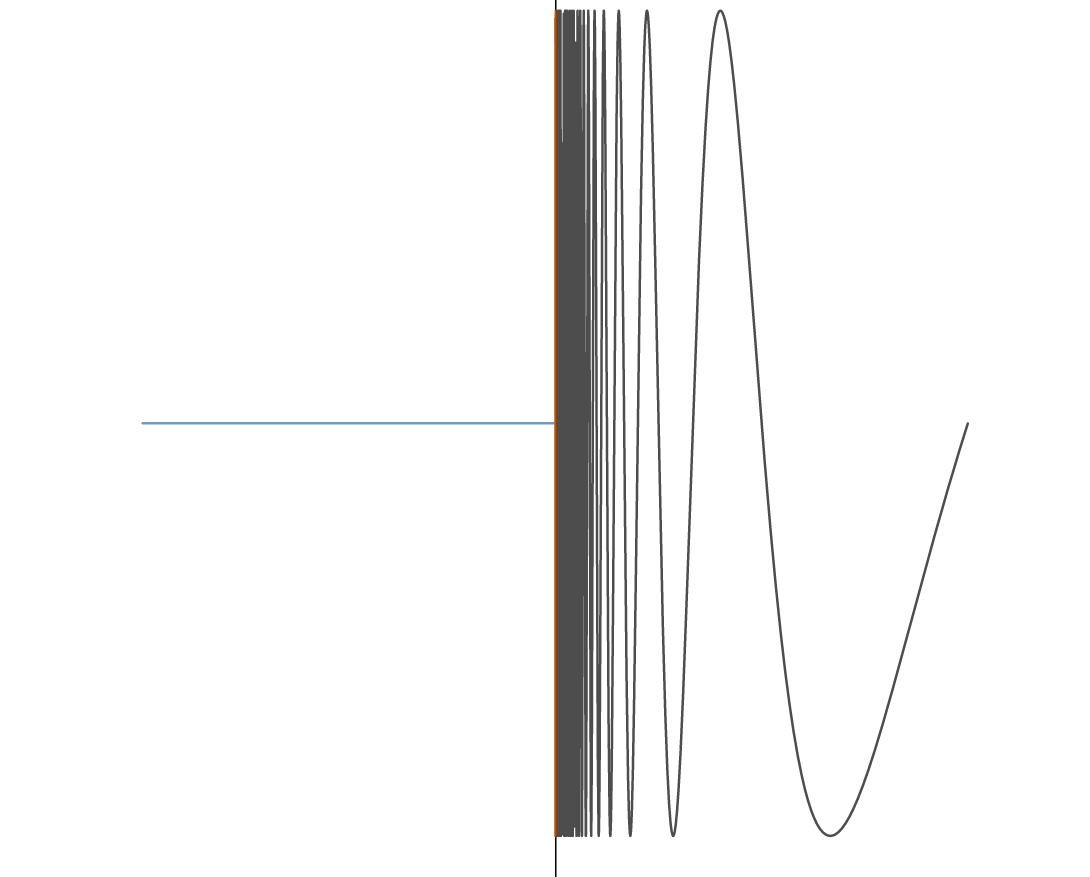
\includegraphics[scale=.2]{images/topint}
		\caption{The Topologist's Interval}
		\label{fig:topint}
	\end{figure}
	
	
	This space is connected, but not path connected, as the vertical stripes become infinitely close near zero, so there is no proper path from a point to the left of the origin to a point to the right.
	
	
	The topologist's circle is the same thing, but with an arc adjoined from $(1,0)$ to $(-1,0)$.
	
	\begin{figure}[!htb]
		\centering
		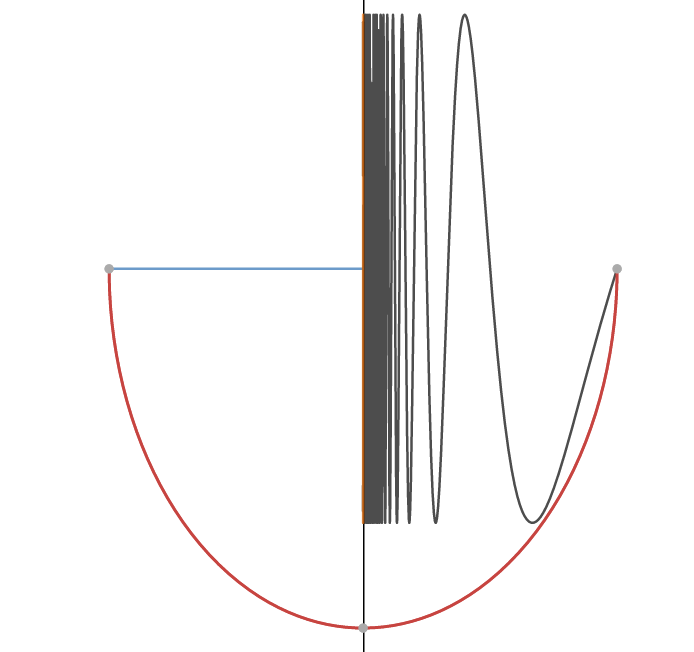
\includegraphics[scale=.3]{images/topcirc}
		\caption{The Topologist's Circle}
		\label{fig:topcirc}
	\end{figure}
	
	This space is connected and path connected, as we can use the arc to avoid the messiness to the right of the origin, but it is not locally path connected, as we can still look at small neighborhoods which look like parallel stripes, and obviously are not path connected.



The subset of $\R^2$ defined piecewise as the union of the closed horizontal segment $[-1,0]$ along the $x$-axis and $y=x\sin(\frac{\pi}{x})$ is locally connected everywhere, but not locally path connected at the origin.


	
	\begin{figure}[!htb]
		\centering
		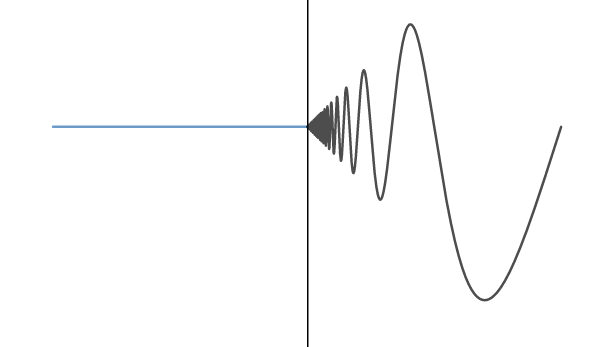
\includegraphics[scale=.3]{images/xsinx}
		\caption{$y=x\sin{\pi/x}$}
		\label{fig:xsinx}
	\end{figure}

}

\thrm{If a space $X$ is path connected, then it is connected.}

